\section{Experimental Difficulties}
\label{sec:nltr-expr-diff}

\subsection{Ferromagnetic Nanorods as a Nonlinear Beacon}

In order to generate a harmonic response, the nonlinear object must possess inherent nonlinearity in its material properties. Since TR uses electromagnetic waves, we are interested in possble nonlinear electric or magnetic properties. In this section, we discuss a potential magnetic nonlinear object in the form of ferromagnetic nanorods. These nanorods have a nonlinear magnetization curve, as shown in ~\todo{add figure for hysteresis loop}. This means that the B-field generated from an interrogation signal should have a harmonic response that we may use for NLTR. 

While the usage of diodes as a nonlinear object had been well-documented, the usage of ferromagnets as a nonlinear object had not. Due to this, we had to perform preliminary experiments on the ferromagnetic nanorods in order to verify that the nonlinear response was strong enough to ensure success NLTR experiments. 

This preliminary expertiment consisted of sending a pulse signal into an antenna with the ferromagnetic nanorods attached to them and recording the response signal. By transforming the response signal to the frequency domain, we were able to easily identify whether or not a 2f harmonic was generated. 
 
 \begin{figure}[h!]
     \centering
     \begin{subfigure}{0.45\textwidth}
         \centering
         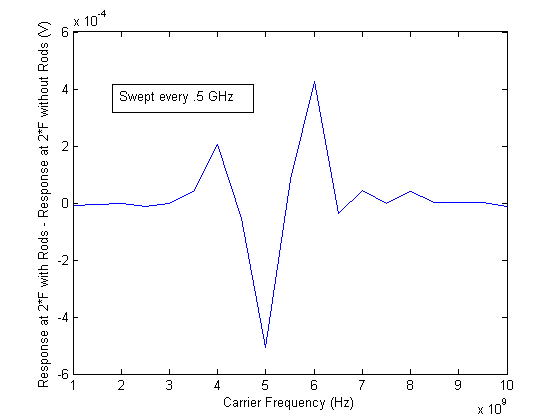
\includegraphics[width=1.0\linewidth]{nanorod/exp-1}
         \caption[]{}
         \label{fig:nanorod-exp-1}
     \end{subfigure}
         \begin{subfigure}{0.45\textwidth}
         \centering
         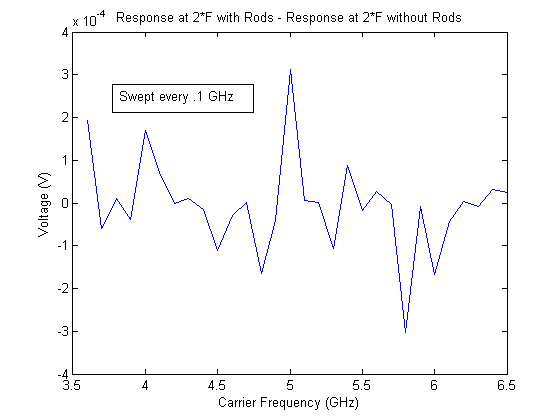
\includegraphics[width=1.0\linewidth]{nanorod/exp-2}
         \caption[]{}
         \label{fig:nanorod-exp-2}
     \end{subfigure}
         \begin{subfigure}{0.45\textwidth}
         \centering
         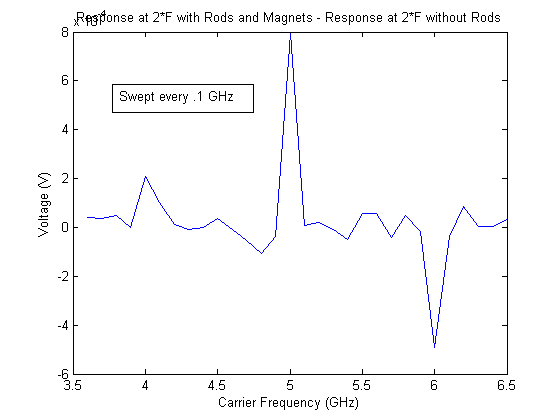
\includegraphics[width=1.0\linewidth]{nanorod/exp-3}
         \caption[]{}
         \label{fig:nanorod-exp-3}
     \end{subfigure}
         \begin{subfigure}{0.45\textwidth}
         \centering
         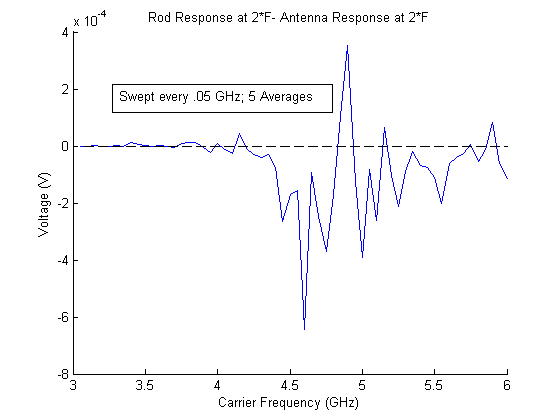
\includegraphics[width=1.0\linewidth]{nanorod/exp-4}
         \caption[]{}
         \label{fig:nanorod-exp-4}
     \end{subfigure}
     \caption[Ferromagnetic nanorod experimental results]{Experimental results}
     \label{fig:nanorod-results}
 \end{figure}
 
  Figure~\ref{fig:nanorod-results}(a)-(d) show the 2f response under a variety of conditions. Although there seem to be peaks in (a) - (d), the peaks are somewhat randomly distributed and are small in magnitude. Due to these two aspects of our preliminary testing, we determined that using ferromagnetic nanorods as a potential magnetic nonlinear object was infeasible for performing NLTR. 
  
\subsection{Diodes as an Electric Nonlinear Beacon}

While utilizing a nonlinear magnetic response was not feasible, utilizing a nonlinear electric response has been well-documented through the use of a diode. This represents a nonlinear object, as the current response to an applied voltage for a diode changes significantly after a certain applied voltage value, as seen in ~\todo{find an image for IV curve-- probably just like Wikipedia}. Frazier et al. have previously used diodes in NLTR experiments to much success.

We performed another preliminary test to verify the nonlinear response of a diode after being interrogated by a Gaussian pulse. Given the history of diodes in NLTR, we believed that we would see a large 2f response. While performing these preliminary tests we were unable to produce any measureable harmonic from a diode while it was present in the Gigabox. In order to circumvent this problem, we used extremely large amplifiers as done by Hong et al. in their NLTR experiments. We were still unable to generate a significant harmonic response.

As a last effort we used various frequency multipliers to generate a nonlinear signal. We did this to verify that the equipment used in our setup was functioning properly. We were able to extract a nonlinear sona from the frequency multiplier; however, this is infeasible in a WPT technology as frequency multipliers are large in size. This confirmed that our equipment was working properly but that we were unable to generate a large response. Due to not being able to generate a nonlinear sona experimentally, we conducted all of our NLTR experiments using numerical simulation.
